\chapter{Criptografia}
\label{cap:criptografia}

A criptologia é a ciência das comunicações secretas \cite{history_of_cryptography_and_cryptanalysis} que contempla diversas técnicas para garantir uma comunicação segura entre um emissor e seu destinatário, através de um canal de comunicação suscetível a interceptações por terceiros não autorizados. A criptologia possui três subáreas: esteganografia, criptografia e criptoanálise. A esteganografia visa ocultar fisicamente uma mensagem, como em áudios, imagens ou papel, sem alterar sua apresentação. A criptografia, por sua vez, altera a apresentação da mensagem, tornando-a ilegível para quem não souber reverter o processo. A criptoanálise é o estudo da segurança dos métodos de criptografia. A Figura \ref{fig:criptologia} ilustra esta divisão de áreas.
 
    \begin{figure}[htb!]
        \centering
        \caption{Representação parcial das áreas da criptologia.}
        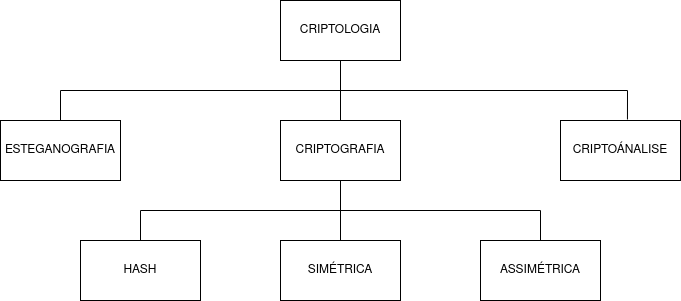
\includegraphics[width=0.75\textwidth]{Figuras/criptologia.png}\\
        \footnotesize{Fonte: O autor.}
        \label{fig:criptologia}
    \end{figure}

A criptografia possui os seguintes objetivos: confidencialidade, integridade, autenticação e irretratabilidade \cite{introduction_to_cryptography}. A confidencialidade visa garantir que um determinado dado possa ser lido apenas por destinatários autorizados. Integridade procura assegurar que um dado não seja modificado durante a transmissão. A autenticação determina que um destinatário possa verificar a origem da mensagem. Por fim, a irretratabilidade certifica que um emissor não possa negar a autoria de uma mensagem. Por si só, um algoritmo de criptografia não assegura estes objetivos e outras necessidades de segurança. Dependendo do cenário, é necessário utilizar diversos algoritmos em conjunto, cada um resolvendo uma parcela do problema. Por exemplo, ao enviar uma mensagem utilizando o \ac{ML-KEM}, iremos garantir apenas confidencialidade e integridade. Para garantir a autenticação e irretratabilidade devemos utilizar um algoritmo de assinatura digital.

Historicamente a criptografia é dividida em dois períodos: criptografia clássica e moderna. Alguns autores como \cite{criptografia_e_seguranca_de_redes,introduction_to_modern_cryptography} consideram a criptografia clássica os métodos de criptografia que antecedem a criação da criptografia assimétrica em 1976 por Whitfield Diffie e Martin Hellman, isto é, métodos de transposição, substituição, \textit{one-time pad}, máquinas de rotor, etc. A Figura \ref{fig:timeline} apresenta alguns dos sistemas de criptografia clássicos e modernos. Entre os anos de 1970 e 1980, a criptografia teve um significativo avanço com a convergência da matemática e computação na área \cite{introduction_to_modern_cryptography}, se destacando a publicação do DES \cite{des} e troca de chaves Diffie-Hellman \cite{diffie-hellman}. A partir desse período, subdisciplinas da matemática, como álgebra abstrata, teoria dos números e matemática finita; e da computação, como teoria da informação e complexidade computacional, passaram a estar presentes na criação e na utilização dos processos de criptografia, assim dando início à criptografia moderna.

    \begin{figure}[htb!]
        \centering
        \caption{Linha do tempo da criptografia.}
        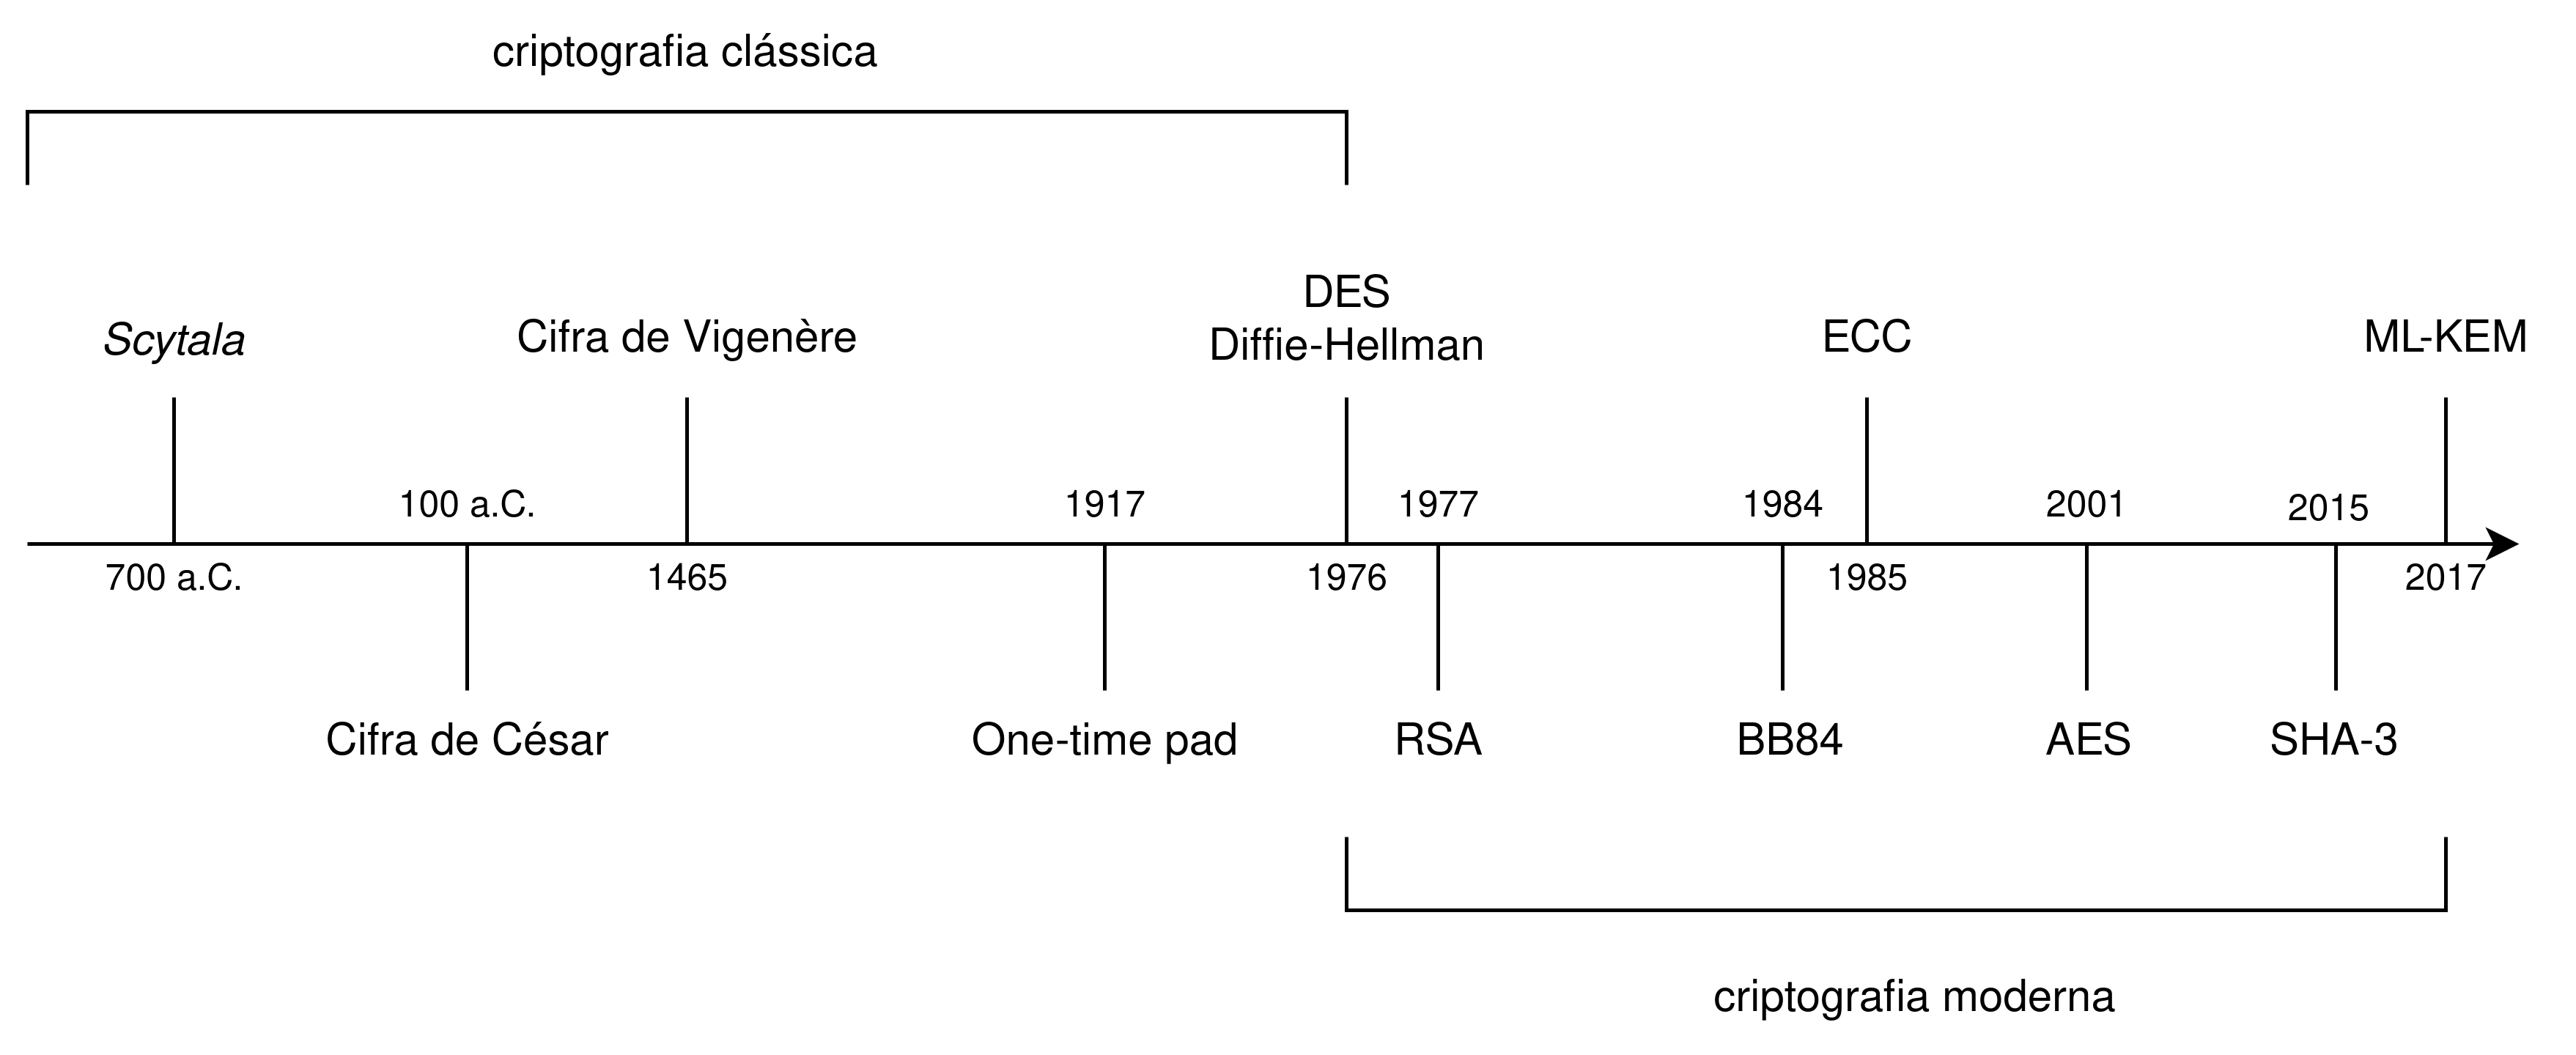
\includegraphics[width=1\textwidth]{Figuras/timeline.png}\\
        \footnotesize{Fonte: O autor.}
        \label{fig:timeline}
    \end{figure}

É importante destacar a diferença entre criptografia quântica e pós-quântica, embora os termos sejam semelhantes e podem causar uma certa confusão, eles se diferem em seu propósito e na natureza de como realizam os processos de criptografia. Os algoritmos quânticos como o BB84, desenvolvido por Charles Bennett e Gilles Brassard \cite{bb84}, utilizam as propriedades da mecânica quântica como método de criptografia. Ou seja, tem como objetivo serem executados em computadores quânticos para garantirem a segurança dos dados. A criptografia pós-quântica é um termo que surgiu devido a preocupação com a segurança das informações criptografadas com algoritmos baseados em problemas que podem ser resolvidos pelo algoritmo de Shor \cite{shor}. Estes algoritmos de criptografia pós-quânticos tem como objetivo serem executados em computadores convencionais, e serem seguros tanto contra ataques realizados por computadores clássicos quanto quânticos \cite{nist}, como é o caso do \ac{ML-KEM}.

A criptografia possui três subáreas principais, as funções \textit{hash}, criptografia simétrica e assimétrica. É importante conhecer as particularidades de cada uma dessas áreas, como, seu funcionamento, s problemas e soluções que os algoritmos destas áreas resolvem. Cada uma delas possui suas vantagens e desvantagens, com isso, são aplicáveis a problemas específicos na criptografia.

\section{Função Hash}
    Uma função \textit{hash} é uma função que mapeia uma entrada de tamanho variável em uma saída de tamanho fixo, $f:\{0,1\}^{*} \rightarrow \{0,1\}^n$. Entretanto, essas funções devem possuir algumas características para serem consideradas funções \textit{hash}:

    \begin{enumerate}
        \item[(i)] saída de tamanho fixo: independente do tamanho da entrada, a saída deve sempre ter o mesmo tamanho;
        \item[(ii)] determinístico: para uma mesma entrada, deve-se sempre obter a mesma saída;
        \item[(iii)] eficiência de operação: a operação de mapeamento deve ser rápida.
    \end{enumerate}

    Funções \textit{hash} não criptográficas são comumente utilizadas onde a segurança dos dados não é uma necessidade, por exemplo, na verificação e integridade de dados, tabelas \textit{hash}, etc. Por sua vez, as funções \textit{hash} criptográficas devem possuir propriedades adicionais para terem aplicabilidade na criptografia, essas propriedades são:

    \begin{enumerate}
        \item[(i)] resistência à pré-imagem: deve ser inviável reverter o processo de \textit{hash}, ou seja, descobrir uma entrada correspondente ao \textit{hash};
        \item[(ii)] resistência à segunda pré-imagem: dado uma entrada e seu \textit{hash}, deve ser difícil achar outra entrada com mesmo \textit{hash};
        \item[(iii)] resistência à colisão: deve ser difícil encontrar duas entradas escolhidas arbitrariamente que possuam o mesmo \textit{hash}.
    \end{enumerate}

    A complexidade de se resolver o problema do item (ii) no pior caso é de $\mathcal{O}(2^n)$, isto porque seria necessário verificar todos os resultados possíveis da função \textit{hash}, até encontrar um resultado compatível com o \textit{hash} de entrada. Já a complexidade de se resolver o problema do item (iii) é de $\mathcal{O}(2^{n/2})$, uma vez que a probabilidade de se encontrar duas mensagens diferentes escolhidas aleatoriamente que produzem o mesmo \textit{hash} é maior que 50\% em $2^{n/2}$ tentativas como demonstrado em \cite{hash_n/2, criptografia_e_seguranca_de_redes}. 

    As funções \textit{hash} criptográficas que possuem as propriedades citadas acima podem ser utilizadas na área da criptografia como, por exemplo, em armazenamento de senhas. Perceba que se fosse aplicada uma função \textit{hash} não criptográfica qualquer a uma senha e armazenada em um banco de dados, a mesma poderia ser decifrada, já que seria possível reverter o processo através da não resistência à pré-imagem. Outras aplicabilidades de funções \textit{hash} são em geradores de números pseudoaleatórios e como subprocessos em outros algoritmos de criptografia.

\section{Criptografia simétrica}
    A criptografia simétrica tem como principal característica a utilização de uma mesma chave criptográfica para a realização dos processos de cifragem e decifragem. Diferente das funções \textit{hash} criptográficas, em que o processo de decifragem não deve ser possível computacionalmente, um algoritmo de criptografia simétrico é projetado para realizar a cifragem e decifragem de uma mensagem usando uma mesma chave criptográfica. Uma mensagem cifrada utilizando um algoritmo simétrico somente pode ser decifrada com a mesma chave que a cifrou. Alguns dos algoritmos de criptografia simétrica mais utilizado é o AES \cite{aes}.

    A Figura \ref{fig:simetrica} ilustra um exemplo da utilização de um algoritmo de cifragem simétrica para o envio de uma mensagem M, no qual C é o algoritmo de cifragem, D é o algoritmo de decifragem, $SK_{AB}$ é a chave simétrica compartilhada entre A e B, e X é a mensagem cifrada.

    \begin{figure}[htb!]
        \centering
        \caption{Envio de mensagem usando criptografia simétrica.}
        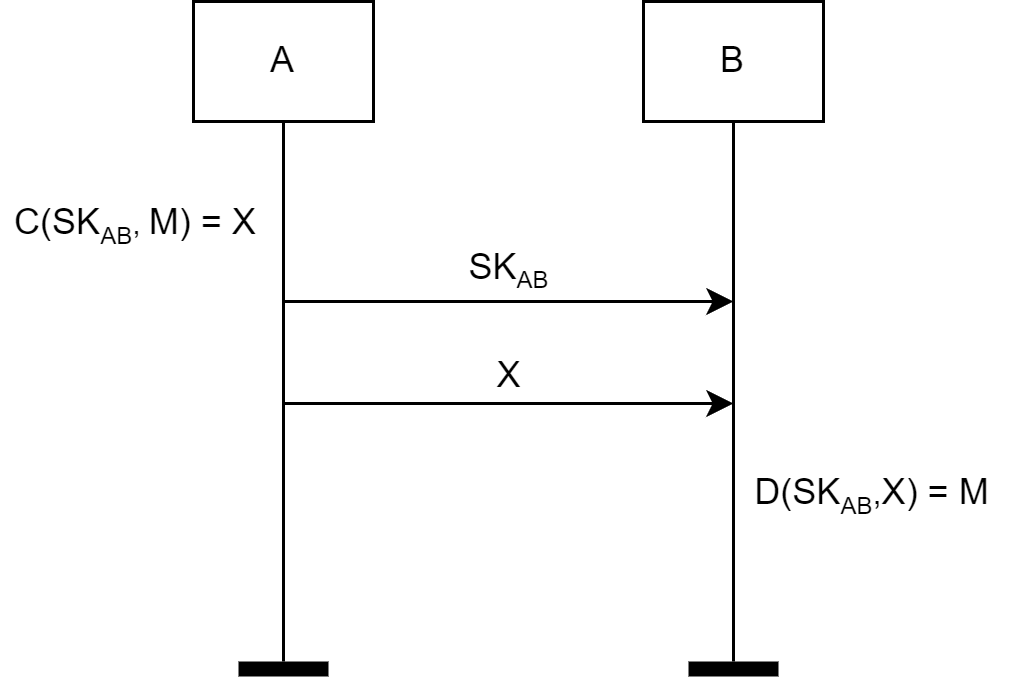
\includegraphics[width=0.65\textwidth]{Figuras/simetrica.png}\\
        \footnotesize{Fonte: O autor.}
        \label{fig:simetrica}
    \end{figure}

    Existem dois tipos de cifras simétricas quanto à forma que uma mensagem é processada: cifras de bloco e cifras em fluxo. As cifras de bloco dividem a mensagem de entrada em blocos de tamanho fixo e processam individualmente cada uma destas, para cada bloco processado se tem um bloco resultante. Caso o tamanho da mensagem não seja divisível pelo tamanho do bloco, é necessário inserir um preenchimento na mensagem de entrada. A cifra AES, por exemplo, pode operar em blocos de 128, 192 ou 256 bits. A Figura \ref{fig:cifra_bloco} ilustra uma cifra de bloco de 128 bits.

    \begin{figure}[htb!]
        \centering
        \caption{Cifra de bloco.}
        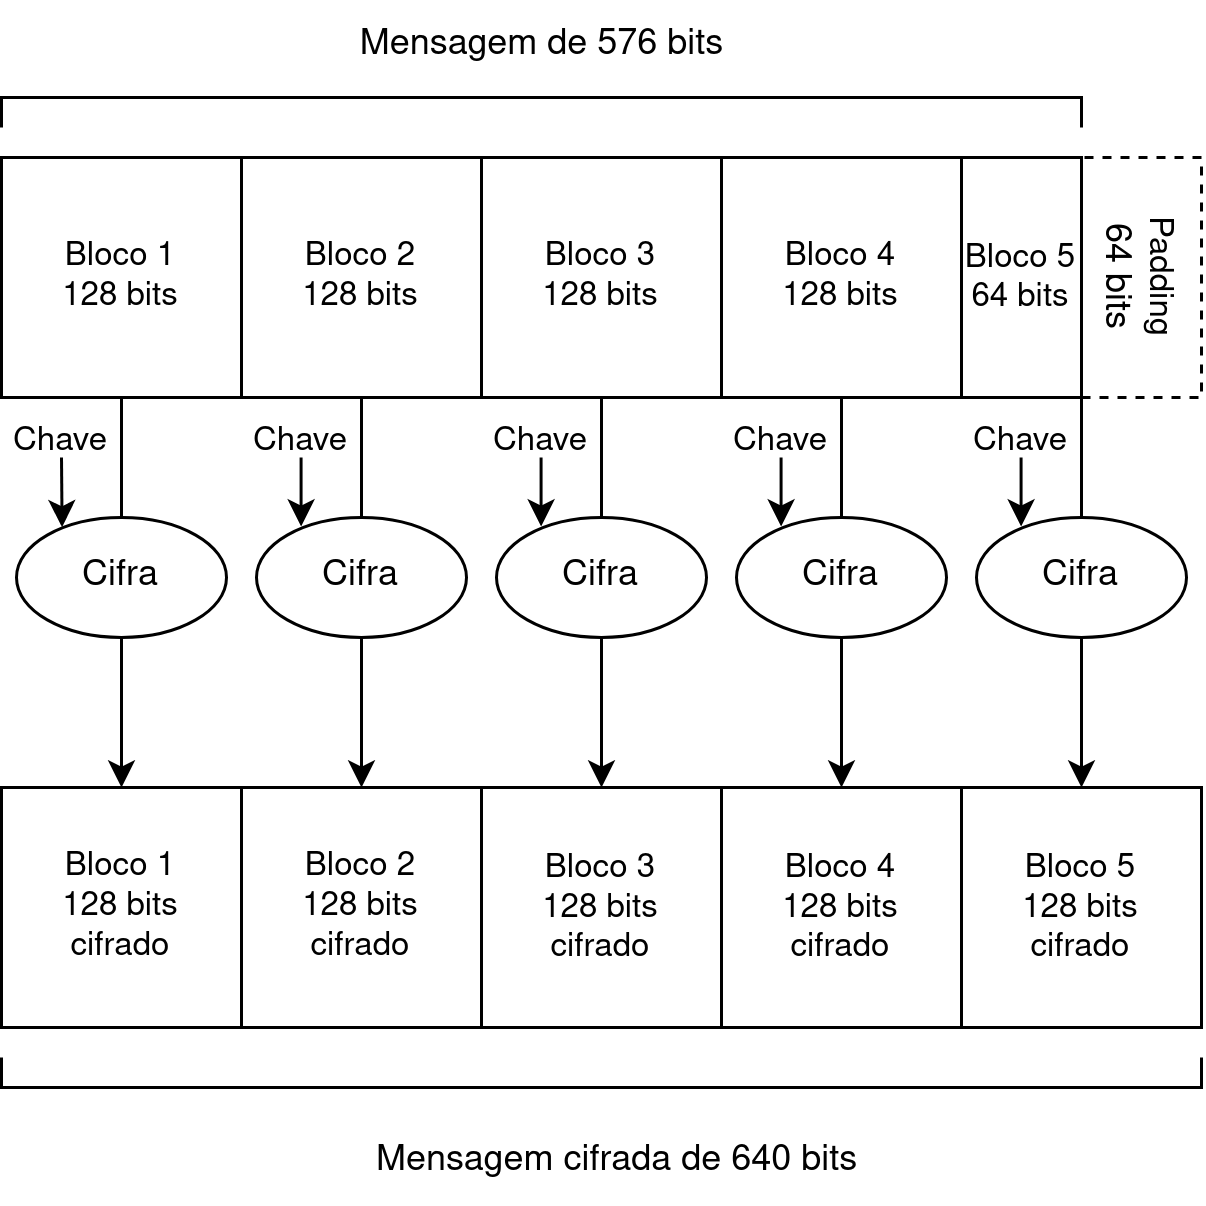
\includegraphics[width=0.65\textwidth]{Figuras/cifra_bloco.png}\\
        \footnotesize{Fonte: O autor.}
        \label{fig:cifra_bloco}
    \end{figure}
    
    As cifras em fluxo, por sua vez, processam os elementos da entrada continuamente, geralmente bit a bit, ou bytes a byte, e produzem uma saída conforme processam esses elementos. A operação $\oplus$ (XOR/ou exclusivo) é um exemplo de cifra de fluxo, na qual a cifragem consiste na aplicação da operação $\oplus$ entre um byte/mensagem e uma chave secreta de um byte,

    \begin{center}
        $\begin{array}{cll}
                   & 10010110 & \textrm{mensagem}\\
            \oplus & 01101100 & \textrm{chave secreta}\\
            \hline
                   & 11111010 & \textrm{mensagem cifrada}
        \end{array}$
    \end{center}

    \noindent
    e a decifragem é realizada simplesmente aplicado novamente a operação $\oplus$ entre o byte cifrado e a mesma chave secreta.
    
    \begin{center}
        $\begin{array}{cll}
                   & 11111010 & \textrm{mensagem cifrada}\\
            \oplus & 01101100 & \textrm{chave secreta}\\
            \hline
                   & 10010110 & \textrm{mensagem}
        \end{array}$
    \end{center}
    
    A principal limitação das cifras simétricas é que, para transmitir uma mensagem cifrada, é necessário também transmitir para a outra parte a chave que decifra esta mensagem, como pode ser visto na Figura \ref{fig:simetrica}. O fato de ter que enviar a chave por um meio de comunicação não seguro, torna necessária a utilização em conjunto com um algoritmo de cifragem assimétrica, onde este tipo de algoritmo possui a particularidade de possuir chaves diferentes para cifrar e decifrar.

    A segurança dos algoritmos de criptografia simétricos não sofreram impacto significativo pela computação quântica. Atualmente, apenas o algoritmo de Grover \cite{grover} reduz a complexidade computacional dos problemas utilizados pelos algoritmos de cifragem simétrica. Em 1996, Lov Grover publicou um algoritmo quântico capaz de realizar a busca de um valor em uma lista de $n$ elementos não ordenados com complexidade $\mathcal{O}(\sqrt{n})$, enquanto computadores clássicos conseguem realizar esta busca em $\mathcal{O}(n)$. Isto significa que um computador quântico pode encontrar uma chave simétrica de 128 bits realizando $2^{64}$ operações com o algoritmo de Grover, ao invés de $2^{128}$ por um computador clássico. Note que para manter a mesma segurança de uma chave simétrica de 128 bits, devemos alterar o tamanho da chave para 256 bits, desta forma um computador quântico terá que realizar $2^{128}$ operações, a mesma quantidade que se tinha com a computação clássica.

\section{Criptografia assimétrica}
    A criptografia assimétrica, também conhecida por criptografia de chave pública, foi inspirada pelo algoritmo de troca de chaves Diffie-Hellman em 1976. Tradicionalmente, para duas partes possuírem a mesma chave simétrica, era necessário que uma delas enviasse sua chave para a outra parte, entretanto, na maioria dos sistemas, não se tem a garantia de um canal de comunicação seguro para essa troca. O algoritmo de Diffie-Hellman \cite{diffie-hellman} foi proposto como uma solução para este problema, estabelecendo uma chave simétrica compartilhada entre duas partes sem a necessidade do envio desta por um meio de comunicação não seguro. O algoritmo de Diffie-Hellman, diferente dos algoritmos simétricos, utiliza dados privados que não devem ser compartilhados, e dados públicos que podem ser compartilhados. No final do processo, ambas as partes possuem uma informação em comum (chave simétrica), que é muito custosa de ser obtida computacionalmente a partir das informações públicas transmitidas pelo meio de comunicação. 
    
    Em 1977, Ron Rivest, Adi Shamir e Leonard Adleman publicaram o primeiro algoritmo de criptografia assimétrica, chamado RSA \cite{rsa}. Diferente do algoritmo de troca de chaves Diffie-Hellman, o RSA realiza a cifragem de mensagens, e não apenas o estabelecimento de uma chave simétrica em comum. Em um algoritmo de criptografia assimétrica como o RSA, a cifragem de uma mensagem somente pode ser realizada por uma chave pública, e a decifragem apenas pela chave privada. Desse modo, o envio de mensagens por um canal de comunicação pode ser realizado de forma segura, já que a chave privada não necessita ser transmitida para outra parte. A Figura \ref{fig:assimetrica} exemplifica esse processo, supondo que A tenha gerado suas chaves públicas e privadas previamente, A envia sua chave pública para B, que por sua vez cifra uma mensagem usando a chave pública de A e envia para A esta mensagem cifrada, A decifra a mensagem com sua chave privada. Assim como o algoritmo Diffie-Hellman, é custoso obter computacionalmente os dados privados a partir dos dados públicos nos algoritmos de criptografia assimétricos.

    \begin{figure}[htb!]
        \centering
        \caption{Envio de mensagem usando criptografia assimétrica.}
        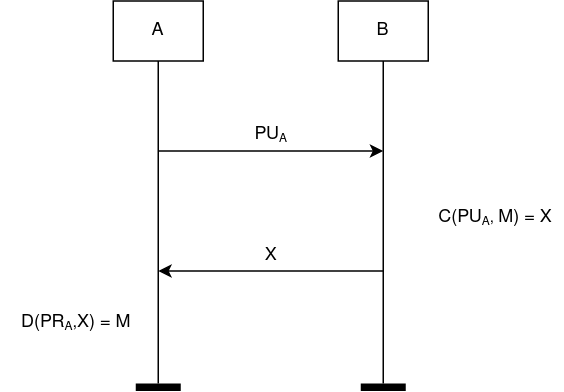
\includegraphics[width=0.65\textwidth]{Figuras/assimetrica.png}\\
        \footnotesize{Fonte: O autor.}
        \label{fig:assimetrica}
    \end{figure}

\section{Encapsulamento de chave}
\label{sec:kem}
    %é mais seguro (CCA2, PKE vs KEM)
    %pegar fontes
    %REFAZER ESTA BOSTA
    %https://www.crypto-textbook.com/download/Understanding-Cryptography-Chapter6.pdf
    Os algoritmos de criptografia assimétricos são projetados para cifrar mensagens de tamanho limitado, enquanto algoritmos simétricos são projetados para cifrar mensagens de tamanho ilimitado. Desta forma, para ser possível a comunicação de longas mensagens entre duas partes utilizando cifra simétrica, é necessária que ambas as partes tenham uma chave simétrica em comum. Atualmente, é utilizado o algoritmo de Diffie-Hellman sob a estrutura algébrica de curvas elípticas \ac{ECDH} para estabelecer esta chave simétrica em comum, entretanto, este algoritmo não é considerado seguro contra computadores quânticos por se basear no problema do logaritmo discreto. Desta forma, é utilizada outra técnica para estabelecer uma chave simétrica comum entre duas partes, chamada \ac{KEM}. A principal diferença entre a troca de chaves Diffie-Hellman e \ac{KEM} é que o algoritmo de Diffie-Hellman não permite a escolha de uma chave privada previamente, esta chave em comum é gerada ao longo do processo. O \ac{KEM}, por sua vez, funciona de uma maneira diferente, uma das partes gera a chave simétrica e a cifra usando a chave pública da outra parte. Desta forma, ambas as partes possuem uma chave simétrica em comum para utilizar em um algoritmo simétrico, e este compartilhamento de chaves é estabelecido por um algoritmo de criptografia assimétrico, neste caso, o algoritmo assimétrico deve ser resistente à computação quântica, como o \ac{ML-KEM}.

    \begin{figure}[htb!]
        \centering
        \caption{Encapsulamento de uma chave privada em comum.}
        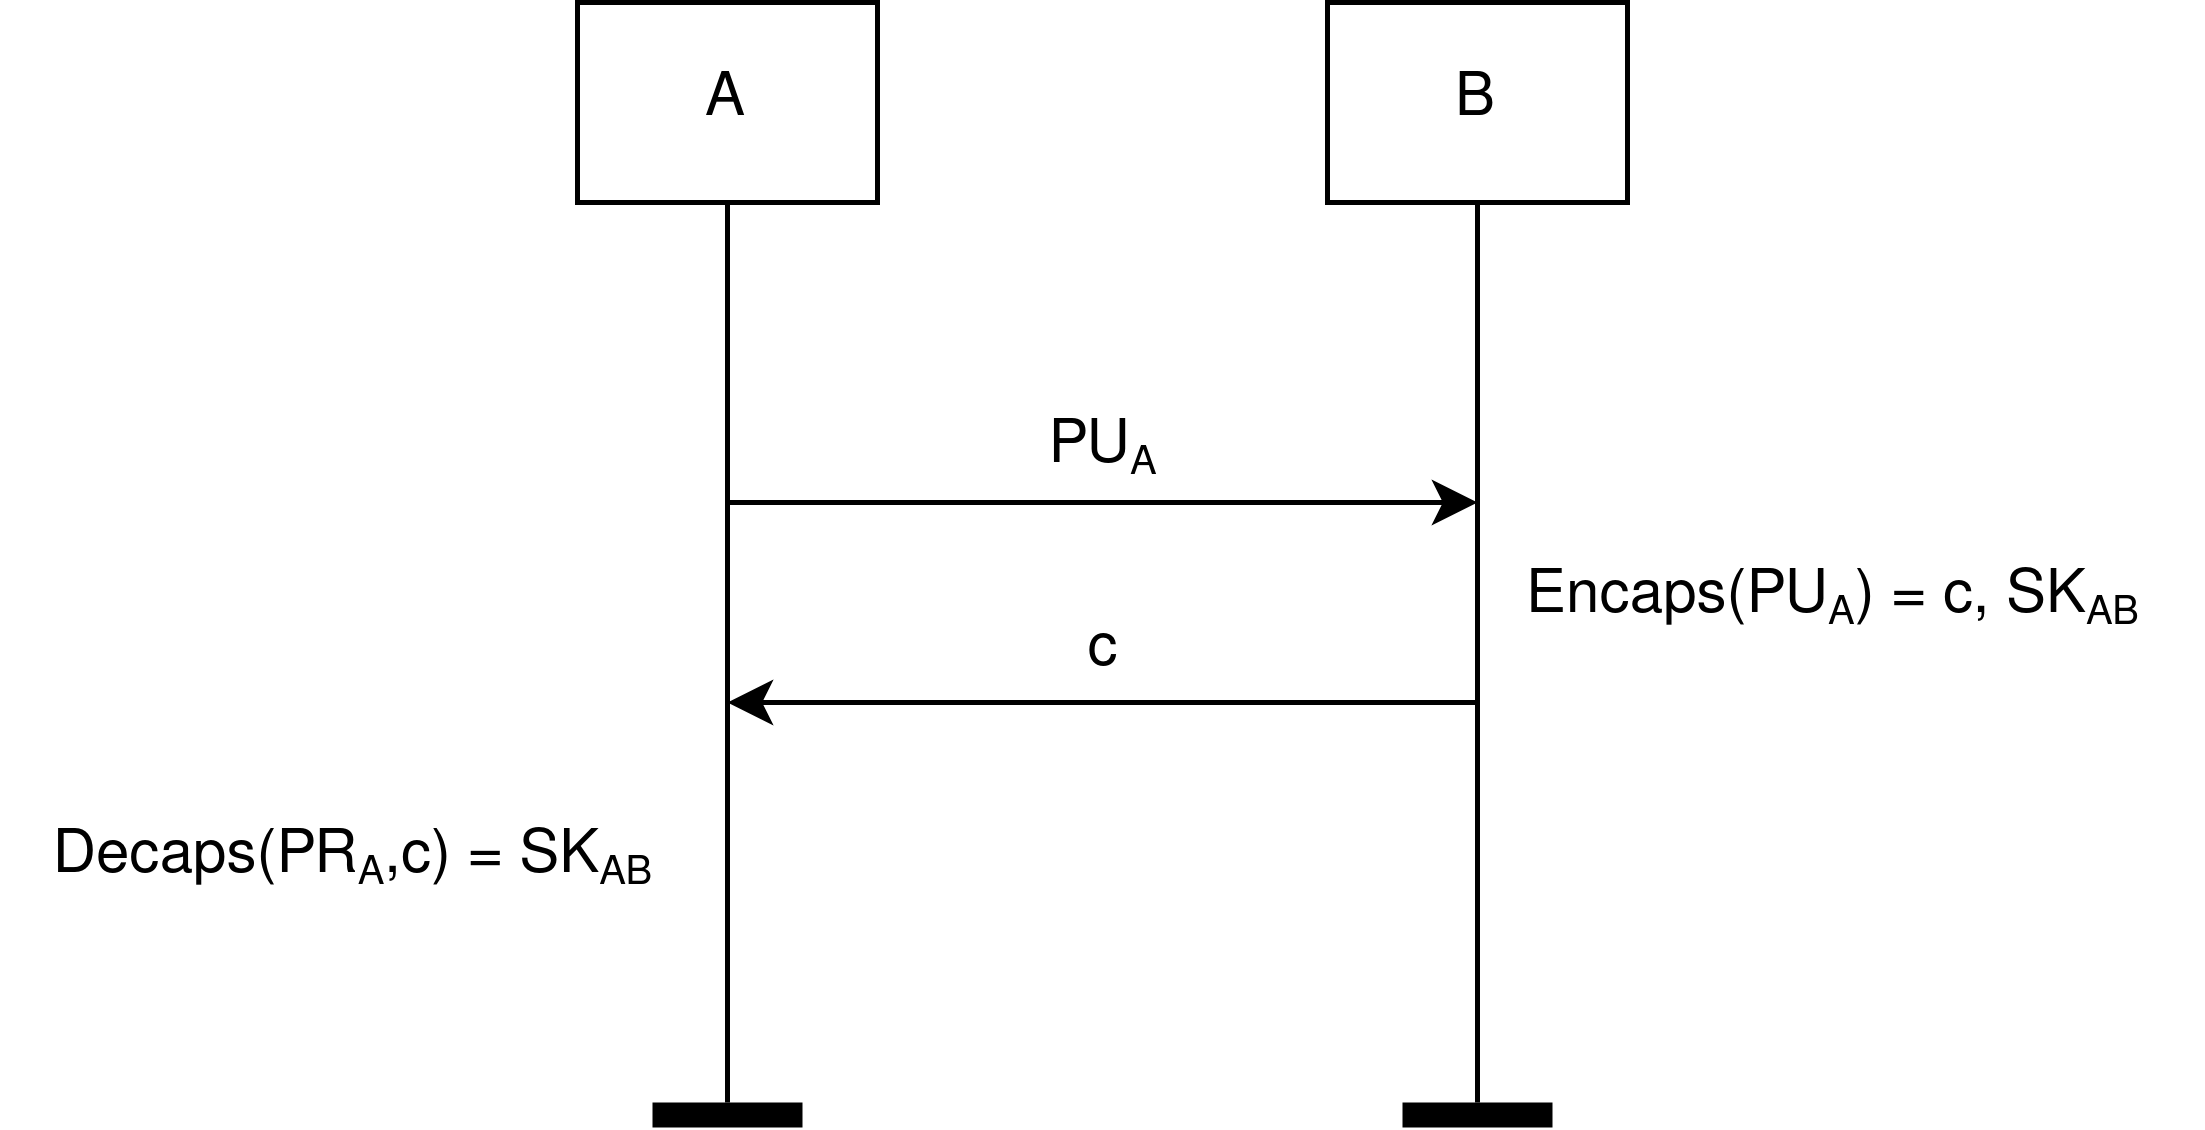
\includegraphics[width=0.75\textwidth]{Figuras/kem.png}\\
        \footnotesize{Fonte: O autor.}
        \label{fig:kem}
    \end{figure}

    O funcionamento do \ac{KEM} pode ser visto na Figura \ref{fig:kem}, na qual A envia sua chave pública $PU_A$ para B, B gera a chave simétrica comum $SK_{AB}$ e a cifra usando a chave pública de A, gerando $c$ que é enviado para A. A, por sua vez, decifra $c$ usando sua chave privada $PR_A$, gerando $SK_{AB}$. 
    
\section{Problemas computacionais}
\label{sec:problemas_computacionais}
    Alguns algoritmos de criptografia assimétrica, como Diffie-Hellman e \ac{ECDH} (Troca de chaves), RSA e \ac{ECC} (Cifragem) e RSA, \ac{ECDSA} e \ac{DSA} (Assinatura digital) possuem sua segurança baseadas nos problemas da fatoração de números inteiros e do logaritmo discreto.

    Eric Bach em \cite{discrete_logarithms_and_factoring_reductions} demonstra uma redução probabilística em tempo polinomial do problema da fatoração prima para o problema do logaritmo discreto e do problema do logaritmo discreto para o problema da fatoração prima. Isso significa que se a fatoração prima de um número $n$ for realizada, então existe uma alta probabilidade de se resolver o problema do logaritmo discreto com módulo $n$ e vice-versa. Isso implica que a complexidade de resolver ambos os problemas algoritmicamente é a mesma, se for desconsiderado o tempo da redução.
    
    A complexidade de se resolver os problemas da fatoração prima e do logaritmo discreto em um computador clássico é $\mathcal{O}(e^{(log\ n)^{1/3}(log\ (log\ n))^{2/3}})$ com o algoritmo \ac{GNFS}, considerado o algoritmo clássico mais eficiente na resolução desses problemas, enquanto o algoritmo de Shor possui a complexidade de $\mathcal{O}((log\ n)^{2}(log\ log\ n)(log\ log\ log\ n))$\cite{shor_vs_gnfs}. A Figura \ref{fig:shor_vs_gnfs} mostra um gráfico comparativo de tempo de execução entre o algoritmo de Shor e \ac{GNFS}.

    \begin{figure}[htb!]
        \centering
        \caption{Comparativo entre os algoritmos Shor e \ac{GNFS} na resolução do problema da fatoração prima de um número composto.}
        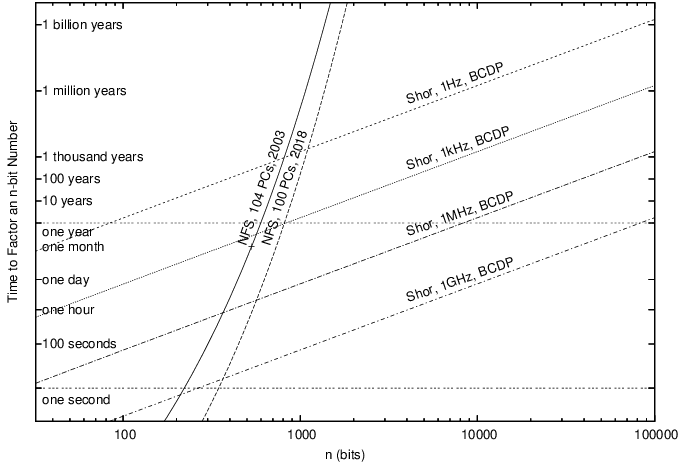
\includegraphics[width=0.75\textwidth]{Figuras/shor_vs_gnfs.png}\\
        \footnotesize{Fonte: \cite{shor_vs_gnfs}.}
        \label{fig:shor_vs_gnfs}
    \end{figure}

        \subsection{Problema da fatoração prima}
        \label{sec:problema_fatoracao_prima}
            O problema da fatoração prima de inteiros consiste em, dado um número composto, encontrar seus fatores primos. Tem-se, como exemplo, de uso de propriedades deste problema, a geração de chaves no sistema de criptografia RSA como pode ser visto no Algoritmo \ref{algo:rsa_gey_gen}. A chave pública $n$ é um número composto gerado pelo produto de dois números primos; fatorando o número $n$, descobrem-se os números primos $p$ e $q$. Obtendo os números $p$ e $q$, pode-se derivar a chave privada completa, visto que o cálculo da chave privada $d$ necessita de $e$, que é uma chave pública, e $\Phi(n)$, que é obtido através de $p$ e $q$.

            \begin{algorithm}[!htbp]
                \SetAlgoLined
                \Saida{Chave pública: $(n,e)$ e Chave privada: $(p,q,d)$}
                Escolha dois números primos $p$ e $q$\\
                Compute $n = p.q$\\
                Compute $\Phi(n) = (p - 1)(q - 1)$\\
                Escolha um expoente $e$ tal que $1 \le e < \Phi(n)$ e $mdc(e,\Phi(n))=1$\\
                Compute $d$ tal que $d.e \equiv 1\ (\textbf{mod}\ \Phi(n))$\\
                \caption{Geração de chaves RSA.}
                \label{algo:rsa_gey_gen}
            \end{algorithm}

            Este é um exemplo de como a existência de um algoritmo que fatora um número composto em tempo polinomial afeta a segurança de um dos principais algoritmos de chave pública utilizados.

        \subsection{Problema do logaritmo discreto}
        \label{sec:problema_logaritmo_discreto}
        
            O problema do logaritmo discreto consiste em, dado um número primo $p$, sua raiz primitiva $r$ e um número $n$ tal que $0 \le n < p$, encontrar o expoente $x$ que satisfaça a equação modular $n \equiv r^x\ (\textbf{mod}\ p)$. Os possíveis valores que satisfazem a equação $n \equiv r^x\ (\textbf{mod}\ p)$ compõem o conjunto finito $\mathbb{Z}_p = \{0,1,2,...,p-1\}$, e a utilização de uma raiz primitiva de $p$ como base faz com que os possíveis resultados sejam uniformemente distribuídos, isto é, de igual probabilidade de serem gerados. Isso faz com que, para encontrarmos o expoente que satisfaça a equação $n \equiv r^x\ (\textbf{mod}\ p)$, seja necessário se verificar todos os possíveis valores de $x$.

            Supondo que um emissor deseja realizar troca de chaves usando o algoritmo de Diffie-Hellmann indicado pelo Algoritmo \ref{algo:diffie-hellman}, resolvendo as equações $A \equiv g^a\ (\textbf{mod}\ p)$ e $B \equiv g^b\ (\textbf{mod}\ p)$ é possível derivar a chave secreta $s$.

            \begin{algorithm}[!htbp]
                \SetAlgoLined
                \Saida{Chave pública: $(p,g,A,B)$, Chave privada lado A: $(a,s)$, Chave privada lado B: $(b,s)$}
                O lado A e B entram em acordo publicamente para utilizar os números primos $p$ e $g$ co-primos, tal que $p > g$.\\
                O lado A escolhe um número $a$ e computa $A = g^a\ \textbf{mod}\ p$\\
                O lado B escolhe um número $b$ e computa $B = g^b\ \textbf{mod}\ p$\\
                Ambos os lados trocam entre si os valores A e B\\
                O lado A computa $s = B^a\ \textbf{mod}\ p$\\
                O lado B computa $s = A^b\ \textbf{mod}\ p$\\
                \caption{Troca de chaves Diffie-Hellman.}
                \label{algo:diffie-hellman}
            \end{algorithm}

            Este é outro exemplo de como um algoritmo que resolve o problema do logaritmo discreto pode afetar um algoritmo de criptografia que baseia sua segurança na dificuldade de se resolver o problema do logaritmo discreto.

\section{Criptoanálise}
    Quando um algoritmo de criptografia é projetado, é necessário um estudo deste algoritmo antes de ser implementado em cenários reais, para que se tenha confiança de sua segurança quando aplicado em dados sensíveis. A subárea da criptologia que visa estudar a segurança de algoritmos de criptografia é a criptoanálise. Devido à variedade de técnicas utilizadas e tipos de criptoanálise, esta seção será restrita apenas a princípios e conceitos básicos desta área, deixando as técnicas de criptoanálise referentes aos algoritmos relacionados a reticulados e ao \ac{ML-KEM} em suas respectivas seções.

    O criptógrafo holandês Auguste Kerckhoffs propôs seis princípios que deveriam ser levados em consideração ao se projetar um criptossistema militar para que este possa ser considerado seguro \cite{kerckhoffs}, são esses princípios:

    \begin{enumerate}
        \item O sistema deve ser materialmente, se não matematicamente, indecifrável;
        \item É necessário que o sistema em si não requeira sigilo, e que não seja um problema se ele cair nas mãos do inimigo;
        \item Deve ser possível comunicar e lembrar da chave sem a necessidade de notas escritas, e os interlocutores devem ser capazes de modificá-la a seu critério;
        \item Deve ser aplicável à correspondência telegráfica;
        \item O sistema deve ser portátil, e não deve exigir a participação de múltiplas pessoas na sua operação e manuseio;
        \item Por fim, o sistema deverá ser simples de usar e não exigir conhecimentos profundos ou concentração dos seus usuários nem um conjunto complexo de regras.
    \end{enumerate}

    Embora esses princípios foram criados para a tecnologia militar da época, eles ainda são válidos para os dias atuais com algumas modificações. Por exemplo, ao invés de dever ser aplicável à correspondência telegráfica, o criptossistema deve ser aplicável aos protocolos de comunicações atuais. O segundo item vai em oposição à segurança por obscuridade, cujo princípio é ocultar todo o funcionamento de um algoritmo, fornecendo o mínimo possível de informações sobre seu funcionamento; dessa forma, acredita-se que quanto menos informações for divulgada sobre o algoritmo de criptografia, mais seguro ele estará. Steven Bellovin e Randy Bush em \cite{obscurity}, argumentam que algoritmos de criptografia que utilizam a obscuridade como técnica para garantir sua segurança podem ser considerados seguros a curto prazo, mas a longo prazo somente os algoritmos publicamente analisados podem ser considerados seguros. Segundo eles, ao se ocultar as vulnerabilidades de um algoritmo de criptografia, as probabilidades de que estas possam ser reparadas diminuem, e aumentam as probabilidades de que estas vulnerabilidades possam ser exploradas por um atacante mal-intencionado. Tornar público o funcionamento de um algoritmo de criptografia permite a análise deste algoritmo pela comunidade científica, assim expondo possíveis vulnerabilidades não descobertas, tornando os algoritmos de criptografia mais seguros e confiáveis. 

    Claude Shannon em \cite{shannon} recomendou que um criptossistema deve possuir duas propriedades, confusão e difusão. O conceito de confusão em uma cifra significa que cada bit do texto cifrado deve depender de uma série de bits da chave criptográfica, dessa forma obscurecendo a relação entre a chave e o texto cifrado, o que dificulta recuperar informações da chave privada a partir do texto cifrado. A propriedade de difusão diz que, se alterado um único bit do texto original, o texto cifrado deve ser alterado em 50\% ou mais, e essas alterações devem estar esparsas no texto cifrado. A ausência desta propriedade significaria que cada bit do texto original estaria relacionado unicamente com um bit do texto cifrado, facilitando um ataque por criptoanálise.
    
    A Tabela \ref{tab:attack_model} mostra alguns modelos de ataques a esquemas de criptografia com base nas informações disponíveis ao criptoanalista, para todos os casos é considerado que o atacante possui conhecimento do algoritmo de cifragem seguindo os princípios de Kerckhoffs. Esses modelos de ataques funcionam como uma espécie de jogo, em que são fornecidas informações ao atacante e, com base nessas informações, o atacante deve ser capaz de recuperar alguma informação útil do texto cifrado. 

    \begin{table}[!htbp]
        \caption{Tipos de ataques a mensagens criptografadas.}
        \centering
        \footnotesize
        \resizebox{\textwidth}{!}{
            \begin{tabular}[h]{|p{5cm}|p{10cm}|}
                \hline
                 Tipo de ataque                & Conhecimento ao criptoanalista \\ \hline
                 Apenas texto cifrado (COA)    & Texto cifrado(desafio)  \\ \hline
                 Texto claro conhecido (KPA)   & Texto cifrado(desafio) e uma ou mais pares de texto claro e texto cifrado por uma chave secreta \\ \hline
                 Texto claro escolhido (CPA)   & Texto cifrado(desafio) e texto claro escolhido juntamente com o texto correspondente cifrado por uma chave secreta  \\ \hline
                 Texto cifrado escolhido (CCA) & Texto cifrado(desafio) e textos cifrados escolhidos juntamente com os textos correspondentes decifrados por uma chave secreta  \\ \hline
                 Texto cifrado escolhido adaptativamente (CCA2) & Texto cifrado(desafio) e textos cifrados escolhidos adaptativamente juntamente com os textos correspondentes decifrados por uma chave secreta  \\ \hline
                 Texto escolhido               & Texto cifrado, texto claro escolhido juntamente com o texto correspondente cifrado por uma chave secreta e texto cifrado pretendido, juntamente com seu texto claro correspondente decifrado por uma chave secreta \\ \hline
            \end{tabular}
        }
        \footnotesize{Fonte: Adaptado de \cite{criptografia_e_seguranca_de_redes}.}
        \label{tab:attack_model}
    \end{table}

    Os modelos de ataques são uma classificação muito utilizada para medir o nível de segurança de esquemas de criptografia. Por exemplo, se foi realizado um ataque malsucedido a um algoritmo de criptografia fornecendo apenas o texto cifrado ao atacante (COA), este algoritmo é considerado menos seguro comparado a outro algoritmo de criptografia que se teve um ataque malsucedido mesmo fornecendo mais informações como pares de textos originais e cifrados (KPA). Note que ambos os algoritmos passaram no teste de criptoanálise, entretanto o segundo algoritmo passou por uma análise mais rígida. 
    
    Outra classificação para esquemas de criptografia é a indistinguibilidade de textos cifrados, essa propriedade garante que, fornecidos pares de textos cifrados e decifrados, o atacante não deve conseguir identificar qual dos textos cifrados corresponde aos textos decifrados com probabilidade maior que 50\% \cite{introduction_to_modern_cryptography}. As três formas de indistinguibilidade de textos cifrados mais usadas na criptografia são:

    \begin{itemize}
        \item \textbf{\textit{Indistinguishability under chosen plaintext attack} (IND-CPA): } O atacante envia um par de textos para um desafiador que cifra um destes textos escolhidos aleatoriamente, e envia este texto cifrado de volta para o atacante, que por sua vez deve deduzir com uma probabilidade maior que 50\% qual dos textos foi cifrado.
        \item \textbf{\textit{Indistinguishability under (non-adaptive) chosen ciphertext attack} (IND-CCA): } O atacante pode realizar cifragens e decifragens de textos escolhidos arbitrariamente por um oráculo, e envia um par de textos para um desafiador que cifra um destes textos escolhidos aleatoriamente, e envia este texto cifrado para o atacante, que por sua vez deve deduzir com uma probabilidade maior que 50\% qual dos textos foi cifrado.
        \item \textbf{\textit{Indistinguishability under adaptive chosen ciphertext attack} (IND-CCA2): } O atacante pode realizar cifragens e decifragens de textos escolhidos arbitrariamente por um oráculo, e envia um par de textos para um desafiador que cifra um destes textos escolhidos aleatoriamente, e envia este texto cifrado para o atacante, que por sua vez pode continuar cifrando e decifrando textos (exceto o texto desafio) utilizando o oráculo para deduzir com uma probabilidade maior que 50\% qual dos textos foi cifrado. 
    \end{itemize}

    No caso do \ac{ML-KEM}, a equipe \ac{CRYSTALS} e o \ac{NIST}, o classificaram como sendo IND-CCA2 seguro \cite{kyber2}, isto significa que mesmo que fornecidos um oráculo de decifragem para um atacante, e permitir que ele realize cifragens e decifragens adaptativamente, ele não ira conseguir recuperar nenhuma informação de uma mensagem cifrada.
    
    Outra classificação para um ataque de criptoanálise segundo \cite{applied_cryptography} é com base na quantidade de recursos computacionais necessários, como a quantidade de processamento, armazenamento e dados para realizar o ataque. Embora exista um método capaz de resolver um problema computacional utilizado em um sistema criptográfico, ou recuperar informações úteis, isso não significa que este ataque seja viável computacionalmente. Por exemplo, é possível descobrir uma senha cifrada por uma função \textit{hash} através de um ataque por força bruta, em que são testadas todas as combinações possíveis, entretanto analisar todas as possibilidades levaria uma quantidade de tempo muito grande. Dessa forma, mesmo que exista uma forma de recuperar a senha por força bruta, esta função \textit{hash} é considerada segura contra este ataque devido ao tempo de processamento necessário. Existem diversos métodos que quebram o \ac{ML-KEM}, mas todos eles demandam muitos recursos computacionais para recuperar alguma informação útil do texto original \cite{kyber2}.

\section{Considerações finais}
    Este capítulo tem a finalidade de fornecer informações essenciais sobre criptografia para que o leitor possa entender o funcionamento do algoritmo \ac{ML-KEM} e assuntos relacionados. São apresentados os principais tipos de criptografia, os problemas da fatoração prima e do logaritmo discreto, estes empregados nos principais algoritmos de criptografia atuais e ameaçados pelo algoritmo de Shor. No Capítulo \ref{cap:reticulados}, é apresentada a estrutura de reticulados, na qual são estabelecidos problemas matemáticos de difícil resolução até mesmo por computadores quânticos, utilizados em algoritmos de criptografia pós-quânticos baseados nesta estrutura.